\begin{name}
	{NGUYÊN HÀM - TÍCH PHÂN}
	{ÔN TẬP CHƯƠNG IV}
	{\tentruong}
	{\thoigian}
\end{name}
\setcounter{ex}{0}\setcounter{bt}{0}
\Opensolutionfile{ans}[ans/ans-2-OTC4-De1]
\caulc
\begin{ex}%[2D4N1-1]
	Hàm số $F(x)$ là một nguyên hàm của hàm số $f(x)$ trên khoảng $K$ nếu
	\choice
	{$F'(x)=-f(x),\,\forall x \in K$}
	{\True $F'(x)=f(x),\,\forall x \in K$}
	{$f'(x)=F(x),\,\forall x \in K$}
	{$f'(x)=-F(x),\,\forall x \in K$}
	\loigiai{
	Theo định nghĩa thì hàm số $F(x)$ là một nguyên hàm của hàm số $f(x)$ trên khoảng $K$ nếu $F'(x)=f(x),\,\forall x \in K$.
	}
\end{ex}
\begin{ex}%[2D4N3-1]
	Cho hai hàm số $y=f(x)$ và $y=g(x)$ liên tục trên đoạn $[a;b]$. Gọi $(\mathscr{D})$ là hình phẳng giới hạn bởi đồ thị hàm số $y=f(x)$ và $y=g(x)$ và hai đường thẳng $x=a,~x=b~(a<b)$. Diện tích của $(\mathscr{D})$ được tính theo công thức nào dưới đây?
	\choice
	{$S=\displaystyle\int\limits_b^a \left| f(x)-g(x)\right|\mathrm{\,d}x$}
	{$S=\displaystyle\int\limits_a^b \left(f(x)-g(x)\right)\mathrm{\,d}x$}
	{\True $S=\displaystyle\int\limits_a^b \left| f(x)-g(x)\right|\mathrm{\,d}x$}
	{$S=\displaystyle\int\limits_a^b f(x)\mathrm{\,d}x-\displaystyle\int\limits_a^b g(x)\mathrm{\,d}x$}
	\loigiai
	{
	Diện tích của $(\mathscr{D})$ được tính theo công thức
	\[S=\displaystyle\int\limits_a^b \left| f(x)-g(x)\right|\mathrm{\,d}x.\]
	}
\end{ex}
\begin{ex}%[2D4N2-1]
	Cho hàm số $f(x)$ liên tục trên $\mathbb{R}$ và $a$ là số thực dương. Khẳng định nào sau đây là khẳng định đúng?
	\choice
	{$\displaystyle\int\limits_a^a f(x) \mathrm{\,d}x=1$}
	{$\displaystyle\int\limits_a^af(x) \mathrm{\,d}x=a^2$}
	{\True $\displaystyle\int\limits_a^af(x) \mathrm{\,d}x=0$}
	{$\displaystyle\int\limits_a^a f(x) \mathrm{\,d}x=2a$}
	\loigiai{
	Gọi $F(x)$ là một nguyên hàm của $f(x)$.
	Ta có $\displaystyle\int\limits_a^af(x) \mathrm{\,d}x=F(x)\Bigg|_a^a=F(a)-F(a)=0$.
	}
\end{ex}
\begin{ex}%[2D4N1-3]
	Họ nguyên hàm của hàm số $f(x) = x^2+\cos x$ là
	\choice
	{$2x-\sin x+C$}
	{\True $\dfrac{1}{3}x^3+\sin x+C$}
	{$x^3+\sin x+C$}
	{$\dfrac{1}{3}x^3-\sin x+C$}
	\loigiai{
	Ta có $\displaystyle \int (x^2+\cos x)\mathrm{\,d}x =\dfrac{1}{3}x^3+\sin x+C$.
	}
\end{ex}
\begin{ex}%[2D4H1-1]
	Nếu $\displaystyle\int f(x) \mathrm{\,d}x=\dfrac{x^3}{3}+e^x+C$, với $C$ là hằng số thì $ f(x) $ là hàm số nào sau đây?
	\choice
	{$f(x)=3x^2+e^x$}
	{$f(x)=\dfrac{x^4}{12}+e^x$}
	{\True $f(x)=x^2+e^x$}
	{$f(x)=\dfrac{x^4}{3}+e^x$}
	\loigiai{
	Theo định nghĩa nguyên hàm thì $f(x)=\left(\dfrac{x^3}{3}+e^x+C\right)'=x^2+e^x$.
	}
\end{ex}
\begin{ex}%[2D4H2-1]
	Cho hàm số $f(x)$ có đạo hàm trên $[-3;5]$. Tính $\displaystyle\int\limits_ {-3}^5 4f'(x)\mathrm{\,d}x$, biết $f(-3)=1$ và $f(5)=9$.
	\choice
	{$I=40$}
	{ $I=36$}
	{$I=8$}
	{\True $I=32$}
	\loigiai{
	Ta có $I=\displaystyle\int\limits_ {-3}^5{4f'(x)\mathrm{\,d}x=4\displaystyle\int\limits_ {-3}^5 {f'(x)\mathrm{\,d}x}=4f(x})\Big|_{-3}^5=4[f(5)-f(-3)]=32$.
	}
\end{ex}
\begin{ex}%[2D4H2-1]
	Biết $\displaystyle\int\limits_1^3f(x)\mathrm{\,d}x=8$. Khi đó kết quả của $\displaystyle\int\limits_1^3\left( 2f(x)-3\right)\mathrm{\,d}x$ bằng
	\choice
	{$16$}
	{\True $10$}
	{$13$}
	{$9$}
	\loigiai{
	$I=\displaystyle\int\limits_1^3[2f(x)-3]\mathrm{\,d}x=\displaystyle\int\limits_1^3 2f(x)\mathrm{\,d}x-\displaystyle\int\limits_1^3 3\mathrm{\,d}x=10$.
	}
\end{ex}
\begin{ex}%[2D4H3-4]
	Cho vật thể $(\mathscr{B})$ giới hạn bởi hai mặt phẳng có phương trình $x=0$ và $x=2$. Cắt vật thể $(\mathscr{B})$ bởi mặt phẳng vuông góc với trục $Ox$ tại điểm có hoành độ bằng $x$, $(0\leq x\leq 2)$ ta được thiết diện có diện tích bằng $x^2(2-x)$. Thể tích của vật thể $(\mathscr{B})$ là
	\choice
	{$V=\dfrac{4}{3}\pi$}
	{\True $V=\dfrac{4}{3}$}
	{$V=\dfrac{2}{3}\pi$}
	{$V=\dfrac{2}{3}$}
	\loigiai{
	Thể tích của vật thể $(\mathscr{B})$ là $V=\displaystyle\int\limits_0^2 x^2(2-x) \mathrm{\,d}x=\displaystyle\int\limits_0^2 (2x^2-x^3) \mathrm{\,d}x=\dfrac{4}{3}$.
	}
\end{ex}
\begin{ex}%[2D4H3-1]
	Diện tích $S$ của hình phẳng giới hạn bởi đồ thị hàm số $y=3x^2+1$, trục hoành và hai đường thẳng $x=0$, $x=2$ là
	\choice
	{$S=12$}
	{$S=8$}
	{$S=9$}
	{\True $S=10$}
	\loigiai{
	Ta có $S=\displaystyle\int\limits_{0}^{2} \big|3x^2+1\big|\mathrm{\,d}x = \displaystyle\int\limits_{0}^{2} (3x^2+1)\mathrm{\,d}x = (x^3+x)\Bigr|^{2}_{0} = 10$.
	}
\end{ex}
\begin{ex}%[2D4H3-3]
	\immini[thm]{Kí hiệu $(\mathscr{H})$ là hình phẳng giới hạn bởi đồ thị hàm số $y=2x-x^2$ và trục $Ox$ (hình bên). Tính thể tích vật thể tròn xoay được sinh ra bởi hình phẳng $(\mathscr{H})$ khi nó quay quanh trục $Ox$.
	\choice
	{$\dfrac{18\pi}{15}$}
	{$\dfrac{17\pi}{15}$}
	{\True $\dfrac{16\pi}{15}$}
	{$\dfrac{19\pi}{15}$}}{
\begin{tikzpicture}[smooth,samples=300,scale=0.8,>=stealth]
	\draw[->] (-2,0)--(3.7,0) node[below]{$x$};
	\draw[->] (0,-2.2)--(0,1.6) node[right]{$y$};
	\draw (0,0) node[above left]{$O$};
	\draw[domain=-0.6:2.6] plot(\x,{-(\x)^2+2*(\x)})node[below]{\scriptsize$y=2x-x^2$};
	\draw[fill=black] (2,0)node[above right]{$2$} circle(1.5pt) (0,0) circle(1pt);
	\fill[pattern=north west lines,smooth] plot[domain=0:2](\x,{-(\x)^2+2*(\x)})--(2,0)--(0,0);
\end{tikzpicture}}
	\loigiai{
	Ta có $2x-x^2=0\Leftrightarrow
	\hoac{
	&x=0\\
	& x=2
	}
	$.\\
	Thể tích cần tìm là
	$V=\pi\displaystyle\int_0^2(2x-x^2)^2\,\mathrm{\,d}x=\dfrac{16\pi}{15}$.}
\end{ex}
\begin{ex}%[2D4V1-6]
	Vi khuẩn E. coli sống chủ yếu ở đường ruột và có số lượng lớn nhất trong hệ vi sinh vật của cơ thể. Một quần thể vi khuẩn E. coli được quan sát trong điều kiện thích hợp, có tốc độ sinh trưởng được cho bởi hàm số $f(t)=480\cdot2^t \ln 2$. Trong đó $t$ tính bằng giờ $(t>0)$, $f(t)$ tính bằng cá thể/giờ. Biết tại thời điểm bắt đầu quan sát, số lượng cá thể được ước tính một cách chính xác khoảng $480$ cá thể. Hàm số biểu thị số lượng cá thể theo thời gian $t$ là
	\choice
	{\True $F(t)=480 \cdot 2^t$}
	{$F(t)=480\cdot2^t+\ln 2$}
	{$F(t)=480 \cdot 2^t-480$}
	{$F(t)=480 \cdot 2^t + 480$}
	\loigiai{
	Gọi $F(t)$ là hàm số biểu thị số lượng các thể theo thời gian $t$. Ta có
	\[F(t)=\displaystyle\int f(t)\mathrm{\,d}t=\displaystyle\int 480\cdot2^t \ln 2\mathrm{\,d}t=480\cdot 2^t +C\]
	Theo giả thiết $F(0)=480 \Rightarrow 480 \cdot 2^0+C=480 \Rightarrow C=0$. Vậy $F(t)=480\cdot2^t$.
	}
\end{ex}
\begin{ex}%[2D4V3-2]
	Người ta muốn đổ bê tông một con đường giới hạn bởi hai đường cong $AB$ và $CD$ (phần gạch sọc) với kích thước như hình vẽ bên dưới.
	\begin{center}
	\begin{tikzpicture}[smooth,samples=300,scale=0.8,>=stealth,x=5cm,y=1.2cm]
	\draw[<->] (0,0)--(2,0);
	\draw[<->] (2.02,1.2)--(2.02,2.2);
	\draw[dashed] (0,-0.4)--(0,2) node[below left]{$A$}--(0,3) node[above left]{$C$}--(0,3.5);
	\draw[dashed] (2,-0.4)--(2,1.2)node[below right]{$B$}--(2,2.2)node[above right]{$D$}--(2,3.5);
	\draw[domain=0:2] plot(\x,{0.2*((\x)^3-3*(\x)^2)+2});
	\draw[domain=0:2] plot(\x,{0.2*((\x)^3-3*(\x)^2)+3});
	\fill[pattern=north west lines,smooth] plot[domain=0:2](\x,{0.2*((\x)^3-3*(\x)^2)+3})--(2,1.2)--plot[domain=2:0](\x,{0.2*((\x)^3-3*(\x)^2)+2});
	\node[below] at (1,0) {$15$ m};
	\node[right] at (2.02,1.7) {\scriptsize$3$ m};
	\end{tikzpicture}
	\end{center}
	Biết rằng đường cong $DC$ nhận được từ đường cong $AB$ bằng cách tịnh tiến theo phương thẳng đứng lên phía trên $3$ m, lớp bê tông cần đổ dày $15 \mathrm{~cm}$ và giá tiền $1 \mathrm{~m}^3$ bê tông là $1\,080\,000$ đồng. Tính số tiền cần dùng để đổ bê tông con đường đó.
	\choice
	{$6\,580\,000$ đồng}
	{\True $7\,290\,000$ đồng}
	{$6\,850\,000$ đồng}
	{$8\,420\,000$ đồng}
	\loigiai{
	Chọn hệ trục toạ độ $Oxy$ như hình vẽ.
	\begin{center}
	\begin{tikzpicture}[smooth,samples=300,scale=0.8,>=stealth,x=5cm,y=1.2cm]
	\draw[->] (0,0)node[below left]{$O$}--(2.2,0)node[below]{$x$};
	\draw[<->] (2.02,1.2)--(2.02,2.2);
	\draw[->] (0,-0.4)--(0,2) node[below left]{$A$}--(0,3) node[above left]{$C$}--(0,4)node[right]{$y$};
	\draw[dashed] (2,-0.4)--(2,1.2)node[below right]{$B$}--(2,2.2)node[above right]{$D$}--(2,3.5);
	\draw[domain=0:2] plot(\x,{0.2*((\x)^3-3*(\x)^2)+2});
	\draw[domain=0:2] plot(\x,{0.2*((\x)^3-3*(\x)^2)+3});
	\fill[pattern=north west lines,smooth] plot[domain=0:2](\x,{0.2*((\x)^3-3*(\x)^2)+3})--(2,1.2)--plot[domain=2:0](\x,{0.2*((\x)^3-3*(\x)^2)+2});
	\node[below] at (1,0) {$15$ m};
	\node[right] at (2.02,1.7) {\scriptsize$3$ m};
	\end{tikzpicture}
	\end{center}
	Khi đó giả sử đường cong $(AB)$ có phương trình $y=f(x)$ thì đường cong $(CD)$ sẽ có phương trình là $y=f(x)+3$.\\
	Diện tích phần cần đổ bê tông là
	$$S=\displaystyle\int\limits_{0}^{15} \big|f(x)+3-f(x)\big|\mathrm{\,d}x = \displaystyle\int\limits_{0}^{15} \big|3\big|\mathrm{\,d}x = 3x\Bigr|^{15}_{0} = 45\,\mathrm{m^2}.$$
	Số tiền cần dùng là $T=45 \cdot 0{,}15 \cdot 1\,080\,000=7\,290\,000$ đồng.
	}
\end{ex}
\Closesolutionfile{ans}
% \indapan{6}{ans/ans-2-OTC4-De1}
\cauds
\Opensolutionfile{ans}[ans/ans-2-OTC4-De1-DS]
\begin{ex}%[2D4H2-2]
	Biết $F(x)=x^3+3x^2$ là một nguyên hàm của hàm số $f(x)$ trên $\mathbb{R}$.
	\choiceTF
	{\True $F(1)=4$}
	{\True $\displaystyle\int\limits_0^1f(x)\mathrm{\,d}x=4$}
	{$f(x)=\dfrac{x^4}{4}+x^3+C$}
	{Nếu $G(x)$ cũng là một nguyên hàm của $f(x)$ trên $\mathbb{R}$ thì $F(x)=G(x)$}
	\loigiai{
	\begin{itemchoice}
	\itemch Thay $x=1$ vào hàm $F(x)=x^3+3x^2$, ta được $F(1)=1^3+3\cdot 1^2=4$.
	\itemch $\displaystyle\int\limits_0^1f(x)\mathrm{\,d}x=F(x)\Bigr|^{1}_{0}=F(1)-F(0)=4-0=4$.
	\itemch Theo định nghĩa nguyên hàm thì $f(x)=F'(x)=3x^2+6x$.
	\itemch Nếu $G(x)$ cũng là nguyên hàm của $f(x)$ trên $\mathbb{R}$ thì $F(x)$ và $G(x)$ sai khác nhau một hằng số $C$, nghĩa là $G(x)=F(x)+C$.
\end{itemchoice}}
\end{ex}
\begin{ex}%[2D4H3-1]
	\immini[thm]{Gọi $S_1$, $S_2$ là diện tích của hai hình phẳng giới hạn bởi đồ thị của hàm số $y=f(x)$ và trục hoành (xem hình vẽ). Biết $S_1=10$ và $S_2=1$.
	\choiceTF
	{\True $\displaystyle\int\limits_{-2}^1f(x)\mathrm{\,d}x=10$}
	{$\displaystyle\int\limits_1^2f(x)\mathrm{\,d}x=1$}
	{$\displaystyle\int\limits_{-2}^2f(x)\mathrm{\,d}x=11$}
	{\True $\displaystyle\int\limits_{-2}^2\left|f(x)\right| \mathrm{\,d}x=11$}
	}{
	\begin{tikzpicture}[scale=.7, font=\footnotesize, line join=round, line cap=round, >=stealth]
	\draw[->] (-2.7,0)--(3,0) node[below left] {$x$};
	\draw[->] (0,-1)--(0,4) node[below left] {$y$};
	\draw[fill=black] (0,0) circle(1pt) node [below right] {$O$};
	\foreach \x in {1,2}
	\fill[black] (\x,0) circle(1pt) node [below] {$\x$};
	\fill[black] (-2,0) circle(1pt) node[above left]{$-2$};
	\path (-1,1) node[fill=white]{$S_1$}
	(1.5,0.65) node{$S_2$}
	;
	\draw[->] (1.5,0.5)--(1.5,-0.2);
	\draw[samples=350,domain=-2.1:2.7,smooth,variable=\x] plot (\x,{(\x+2)*(\x-1)*(\x-2)/2})node[above ]{$y=f(x)$};
	\draw[pattern=north east lines,opacity=0.5] (-2,0)plot[domain=-2:2] (\x,{(\x+2)*(\x-1)*(\x-2)/2})--(2,0)--cycle;
	\end{tikzpicture}
	}
	\loigiai{
	Dựa theo ý nghĩa hình học của tích phân thì
	\begin{itemchoice}
	\itemch $\displaystyle\int\limits_{-2}^1f(x)\mathrm{\,d}x=S_1=10$.
	\itemch $\displaystyle\int\limits_1^2f(x)\mathrm{\,d}x=-S_2=-1$.
	\itemch $\displaystyle\int\limits_{-2}^2f(x)\mathrm{\,d}x=S_1-S_2=9$.
	\itemch $\displaystyle\int\limits_{-2}^2\left|f(x)\right| \mathrm{\,d}x=S_1+S_2=11$.
	\end{itemchoice}
	}
\end{ex}
\begin{ex}%[2D4V1-6]
	Tại một khu di tích vào ngày lễ hội hàng năm, tốc độ thay đổi lượng khách tham quan được biểu diễn bằng hàm số $Q'(t)=4 t^3-72 t^2+288t$, trong đó $t$ tính bằng giờ $(0 \leq t \leq 13)$, $Q'(t)$ tính bằng khách/giờ (Nguồn: R. Larson and B. Edwards, Calculus 10e, Cengage). Sau $2$ giờ đã có $500$ người có mặt.
	\choiceTF
	{Lượng khách tham quan được biểu diễn bởi hàm số $Q(t)=t^4-24 t^3+144 t^2$}
	{\True Sau $5$ giờ lượng khách tham quan là $1325$ người}
	{Lượng khách tham quan lớn nhất là $1296$ người}
	{Tốc độ thay đổi lượng khách tham quan lớn nhất tại thời điểm $t=6$}
	\loigiai{
	\begin{itemchoice}
	\itemch Ta có \[Q(t)=\displaystyle\int Q'(t)\mathrm{\,d}t=t^4-24t^3+144t^2+C.\]
	Sau $2$ giờ có $500$ người, nghĩa là $Q(2)=500$. Suy ra $C=100$.\\
	Vậy $Q(t)=t^4-24 t^3+144 t^2+100$.
	\itemch Lượng khách tham quan sau $5$ giờ là $Q(5)=1\,325$ người.
	\itemch Bài toán trở thành tìm giá trị lớn nhất của hàm $Q(t)$ trên $[0;13]$. Ta có
	\begin{itemize}
	\item [$\bullet$] $Q'(t)=0 \Leftrightarrow$ $t=0$, $t=6$ và $t=12$;
	\item [$\bullet$] Tính được $Q(0)=100$, $Q(6)=1\,396$, $Q(12)=100$, $Q(13)=269$.
	So sánh các giá trị này, ta được $Q_{\max}=Q(6)=1\,396$ (người).
	\end{itemize}
	\itemch Bài toán trở thành tìm giá trị lớn nhất của hàm $Q'(t)$ trên $[0;13]$. Ta có
	\begin{itemize}
	\item [$\bullet$] $Q''(t)=12t^2-144t+288$, $Q''(t)=0 \Leftrightarrow$ $t_1=6-2\sqrt{3}$, $t_2=6+2\sqrt{3}$.
	\item [$\bullet$] Bảng biến thiên của hàm $Q'(t)$ trên $[0;13]$ là
	\begin{center}
	
\begin{tikzpicture}
	\tkzTabInit[lgt=1.4,espcl=3]
	{$t$ /0.7, $Q''(t)$ /0.7, $Q'(t)$ /2.5}
	{$0$,$6-2\sqrt{3}$,$6+2\sqrt{3}$,$13$}
	\tkzTabLine{,+,$0$,-,$0$,+,}
	\tkzTabVar{-/$0$,+/$Q'(t_1)$,-/$Q'(t_2)$,+/$364$}
	\end{tikzpicture}
	\end{center}
	Do $Q'(t_1)\approx332{,}6<Q'(13)$ nên $Q'_{\max}$ tại thời điểm $t=13$.
	\end{itemize}
	\end{itemchoice}
	}
\end{ex}
\begin{ex}%[2D4V2-6]
	\immini[thm]{ Một vật chuyển động trong $4$ giờ với vận tốc $v$ (km/h) phụ thuộc
	thời gian $t$ (h) có đồ thị của vận tốc như hình bên. Trong khoảng thời gian $3$ giờ kể từ khi bắt đầu chuyển động, đồ thị đó là một phần của đường parabol có đỉnh $I(2;9)$ với trục đối xứng song song với trục tung, khoảng thời gian còn lại đồ thị là một đoạn thẳng song song với trục hoành.
	\choiceTF
	{\True Vận tốc lớn nhất của chuyển động là $9$ (km/h)}
	{\True $v(t)=-\dfrac{9}{4}t^2+9t$, với $0 \le t \le 3$}
	{$v(t)=\dfrac{27}{4}t$, với $3 \le t \le 4$}
	{\True Quãng đường vật di chuyển được trong $4$ giờ là $27$ km}
	}{
	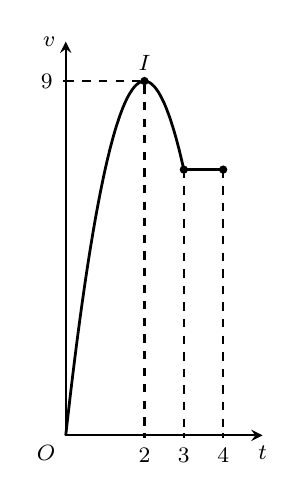
\begin{tikzpicture}[>=stealth,x=1.0cm,y=1.0cm,scale=0.5,thick]
	\draw[<->] (0,10) node[left]{\footnotesize $v$}--(0,0)--(5,0) node[below] {\footnotesize $t$};
	\foreach \x in {2,3,4}
	\draw[shift={(\x,0)},color=black] (0pt,2pt) -- (0pt,-2pt) node[below] {\footnotesize $\x$};
	\foreach \y in {9}
	\draw[shift={(0,\y)},color=black] (2pt,0pt) -- (-2pt,0pt) node[left] {\footnotesize $\y$};
	\draw (0,0) node[below left] {\footnotesize $O$};
	\draw[line width=1.0pt,color=black,smooth,domain=0:3] plot(\x,{-9*(\x)^2/4+9*\x});
	\draw[dashed] (0,9)--(2,9)--(2,0) (3,6.75)--(3,0) (4,6.75)--(4,0);
	\draw[line width=1.0pt,color=black] (3,6.75)--(4,6.75);
	\fill[black] (2,9) circle[radius=3pt] node[above]{\footnotesize $I$}(3,6.75) circle[radius=3pt] (4,6.75) circle[radius=3pt];
	\end{tikzpicture}
	}
	\loigiai{
	\begin{itemchoice}
	\itemch Dựa vào đồ thị của hàm vận tốc trên miền $t \in [0;4]$ thì $v_{\max}=9$ (km/h) khi $t=2$.
	\itemch Trên đoạn $t \in [0;3]$ thì đồ thị $v(t)$ là một parabol có đỉnh là $I(2;9)$ nên phương trình của nó có dạng $y=a(t-2)^2+9.$ Do parabol đi qua gốc tọa độ nên \[a(0-2)^2+9=0 \Leftrightarrow 4a+9=0 \Leftrightarrow a =-\dfrac{9}{4}.\]
	Vậy trên đoạn $[0;3]$ thì $v(t)=-\dfrac{9}{4}t^2+9t$.
	\itemch Với $t=3$ thì $v=\dfrac{27}{4}$. Trên đoạn $t \in [3;4]$ thì phần đồ thị là đường thẳng song song với trục hoành, suy ra $v(t)=\dfrac{27}{4}$ khi $t \in[3;4]$.
	\itemch Quãng đường mà vật di chuyển được trong $4$ giờ là
	$$s=\displaystyle\int\limits_0^3 \left (-\dfrac{9}{4}t^2+9t \right )\mathrm{\, d}t+\int\limits_3^4\dfrac{27}{4}\mathrm{\, d}t=27 \,\text{km}. $$
	\end{itemchoice}
	}
\end{ex}
\Closesolutionfile{ans}
% \indapan{2}{ans/ans-2-OTC4-De1-DS}
\caukq
\Opensolutionfile{ans}[ans/ans-2-OTC4-De1-KQ]
\begin{ex}%[2D4H1-2]
	Cho $F(x)$ là một nguyên hàm của hàm số $f(x)=\dfrac{1}{x^2}$ thỏa mãn $F(2)=\dfrac{3}{2}$. Tính $F(1)$.
	\shortans{$1$}
	\loigiai{
	Ta có $F(x)=\displaystyle\int f(x)\mathrm{\,d}x= -\dfrac{1}{x}+C$. Vì $F(2)=\dfrac{3}{2}$ nên $-\dfrac{1}{2}+C=\dfrac{3}{2}\Leftrightarrow C=2$.\\
	Do đó, $F(x)=-\dfrac{1}{x}+2$.	Suy ra $F(1)=-\dfrac{1}{1}+2=1$.
	}
\end{ex}
\begin{ex}%[2D4V2-2]
	Cho hàm số $f(x)=\heva{&x^2+1 & \text{ nếu } x\geq 1\\&2x & \text{ nếu } x<1}$. Tính tích phân $\displaystyle\int\limits_0^2 f(x)\mathrm{\,d}x$ (\textit{làm tròn đến hai chữ số thập phân}).
	\shortans{$4{,}33$}
	\loigiai
	{Vì $\lim\limits_{x \to 1^+} f(x) = \lim\limits_{x \to 1^-} f(x)=f(1)=2$ nên hàm số $f(x)$ liên tục trên $\mathbb{R}$.\\
	Vì vậy $\displaystyle\int\limits_0^2 f(x)\mathrm{\,d}x = \displaystyle\int\limits_0^1 2x\mathrm{\,d}x + \displaystyle\int\limits_1^2 \left(x^2+1\right)\mathrm{\,d}x =1+ \dfrac{10}{3} = \dfrac{13}{3}\approx 4{,}33$.}
\end{ex}
\begin{ex}%[2D4H3-1]
	Tính diện tích $S$ của hình phẳng giới hạn bởi các đường $y=\mathrm{e}^x$, $y=2$, $x=0$, $x=1$ (\textit{làm tròn đến hai chữ số thập phân}).
	\shortans{$0{,}49$}
	\loigiai{
	Xét $\mathrm{e}^x=2 \Leftrightarrow x=\ln 2$.\\
	Diện tích hình phẳng giới hạn bởi các đường $y=\mathrm{e}^x$, $y=2$, $x=0$, $x=1$ là
	\begin{eqnarray*}
	S=\displaystyle\int_{0}^{1}\left|\mathrm{e}^x-2\right|\mathrm{\,d}x
	&=&\displaystyle\int_{0}^{\ln 2}\left|\mathrm{e}^x-2\right|\mathrm{\,d}x+\displaystyle\int_{\ln 2}^{1}\left|\mathrm{e}^x-2\right|\mathrm{\,d}x\\
	&=&-\displaystyle\int_{0}^{\ln 2}\left(\mathrm{e}^x-2\right)\mathrm{\,d}x+\displaystyle\int_{\ln 2}^{1}\left(\mathrm{e}^x-2\right)\mathrm{\,d}x\\
	&=& -\left.\left(\mathrm{e}^x-2x\right)\right|_0^{\ln 2}+\left.\left(\mathrm{e}^x-2x\right)\right|_{\ln 2}^{1}\\
	&=& -(2-2\ln 2-1)+(\mathrm{e}-2-2+2\ln 2)\\
	&=&4\ln 2+\mathrm{e}-5\approx 0{,}49.
	\end{eqnarray*}
	}
\end{ex}
\begin{ex}%[2D4V2-6]
	Giá trị trung bình của hàm số liên tục $f(x)$ trên đoạn $[a ; b]$ được định nghĩa là
	$$
	\dfrac{1}{b-a} \int_a^b f(x) \mathrm{\,d}x .
	$$
	Giả sử nhiệt độ ngoài trời ở một thành phố vào các thời điểm khác nhau trong ngày được mô phỏng bởi công thức $	h(t)=29+3 \sin \left[\dfrac{\pi}{12}(t-9)\right]$, với $h$ tính bằng độ $\mathrm{C}$ và $t$ là thời gian trong ngày tính bằng giờ.	Tìm nhiệt độ trung bình (đơn vị: độ) của ngày trong khoảng thời gian từ $6$ giờ sáng đến $12$ giờ trưa.
	\shortans{$29$}
	\loigiai{
	Nhiệt độ trung bình của ngày trong khoảng thời gian $6\le t \le 12$ được tính bởi công thức sau
	\begin{align*}
		\dfrac{1}{12-6} \int_6^{12} h(t) \mathrm{\,d}t
		&=\dfrac{1}{6} \int_6^{12} \left( 29+3 \sin \left[\dfrac{\pi}{12}(t-9)\right]\right) \mathrm{\,d}t\\
		&=29.
	\end{align*}
}
\end{ex}
\begin{ex}%[2D4C2-6]
Tại một nhà máy sản xuất một loại phân bón, gọi $P(x)$ là lợi nhuận (tính theo triệu đồng) thu được từ việc bán $x$ tấn sản phẩm trong một tuần. Khi đó, đạo hàm $P^{\prime}(x)$, gọi là lợi nhuận cận biên, cho biết tốc độ tăng lợi nhuận theo lượng sản phẩm bán được. Giả sử lợi nhuận cận biên (tính theo triệu đồng trên tấn) của nhà máy được ước lượng bởi công thức
$$
P^{\prime}(x)=16-0{,}02 x \text { với } 0 \leq x \leq 100.
$$
Tính lợi nhuận (triệu đồng) nhà máy thu được khi bán $90$ tấn sản phẩm trong tuần. Biết rằng nhà máy lỗ $25$ triệu đồng nếu không bán được lượng sản phẩm nào trong tuần.
	\shortans{$1334$}
\loigiai{
	Ta có $P(0)=-25$ (lỗ khi không bán được lượng sản phẩm nào trong tuần)
	\allowdisplaybreaks
	\begin{align*}
	P(90)-P(0) &=\displaystyle\int\limits_0^{90} P^{\prime}(x) \mathrm{\,d}x=\displaystyle\int\limits_0^{90}(16-0{,}02 x) \mathrm{\,d} x \\
	&=16 \displaystyle\int\limits_0^{90} \mathrm{\,d} x-0{,}02 \displaystyle\int\limits_0^{90} x \mathrm{\,d} x \\
	&=\left.16 x\right|_0 ^{90}-0{,}01 x^2\left.\right|_0 ^{90}=1359.
	\end{align*}
	Suy ra $P(90)=P(0)+1359=-25+1359=1334$ (triệu đồng).\\
	Vậy lợi nhuận nhà máy thu được khi bán $90$ tấn sản phẩm trong tuần là $1334$ triệu đồng.
}
\end{ex}
\begin{ex}%[2D4C3-3]
	\immini[thm]
	{Gọi $(\mathscr{H})$ là hình phẳng giới hạn bởi đồ thị $(\mathscr{C})$ của hàm số $y=\sqrt{x}$, trục $Ox$ và đường thẳng $x=9$. Cho điểm $M$ thuộc đồ thị $(\mathscr{C})$ và điểm $A(9;0)$. Gọi $V_1$ là thể tích khối tròn xoay tạo thành khi hình phẳng $(\mathscr{H})$ quay quanh trục $Ox$, $V_2$ là thể tích khối tròn xoay tạo thành khi tam giác $OMA$ quay quanh trục $Ox$.\\
	Biết rằng $V_1=2V_2$. Tính diện tích $S$ phần hình phẳng giới hạn bởi đồ thị $(\mathscr{C})$ và đường thẳng $OM$ (\textit{làm tròn đến hàng phần trăm}).
	\shortans{$2{,}92$}
	}
	{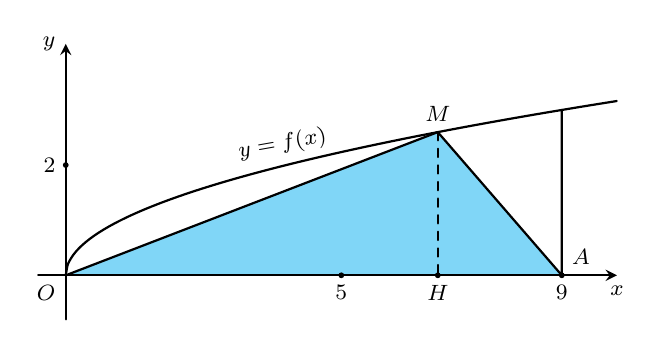
\begin{tikzpicture}[>=stealth,scale=0.7, line join=round, line cap=round,thick,font=\footnotesize]
	\def\xt{-0.5} \def\xp{10} \def\yt{4.2} \def\yd{-0.8}
	\fill[cyan!50!white](0,0)--(6.75,2.598)--(9,0)--cycle;
	\draw[->] (\xt,0)--(\xp,0) node [below]{$x$};
	\draw[->] (0,\yd)--(0,\yt) node [left]{$y$};
	\node at (0,0) [below left]{$O$};
	\node at (4,2) [above,rotate=10] {$y=f(x)$};
	\fill (0,2)node [left]{$2$} circle(1.5pt);
	\foreach \x in {5,9} \fill (\x,0)node[below]{$\x$} circle(1.5pt);
	\draw[smooth,samples=300,domain=0:10] plot(\x,{sqrt(\x)});
	\draw (0,0)--(6.75,2.598)--(9,0)--(9,3);
	\draw[dashed](6.75,2.598)--(6.75,0);
	\fill (6.75,2.598)node[above]{$M$} (9,3) (6.75,0)node[below]{$H$} circle(1.5pt);
	\node at (9,0)[above right]{$A$};
	\end{tikzpicture}}
	\loigiai
	{Theo bài ra ta có $V_1=\pi\displaystyle\int\limits_{0}^{9}(\sqrt{x})^2\mathrm{\,d}x=\dfrac{81\pi}{2}$.\\
	Gọi $H$ là hình chiếu vuông góc của $M$ trên trục $Ox$.\\
	Đặt $OH=m$ (với $0<m<9$), khi đó $M(m;\sqrt{m})$, $MH=\sqrt{m}$, $AH=9-m$.\\
	Suy ra
	\[V_2=\dfrac{1}{3}\pi\cdot MH^2\cdot OH + \dfrac{1}{3}\pi\cdot MH^2\cdot AH = \dfrac{1}{3}\pi\cdot MH^2\cdot OA = 3m\pi.\]
	Theo giả thiết $V_1=2V_2$ nên $\dfrac{81\pi}{2}=6m\pi \Leftrightarrow m=\dfrac{27}{4}$. Do đó $M\left(\dfrac{27}{4};\dfrac{3\sqrt{3}}{2}\right)$.\\
	Phương trình đường thẳng $OM$ là $y=\dfrac{2\sqrt{3}}{9}x$.\\
	Vậy diện tích hình phẳng giới hạn bởi đồ thị $(C)$ và đường thẳng $OM$ là
	$$S=\displaystyle\int\limits_{0}^{\tfrac{27}{4}} \left(\sqrt{x} - \dfrac{2\sqrt{3}}{9}x\right)\mathrm{\,d}x = \left(\dfrac{2}{3}x\sqrt{x}-\dfrac{\sqrt{3}}{9}x^2\right)\Bigg|_{0}^{\tfrac{27}{4}} = \dfrac{27\sqrt{3}}{16} \approx 2{,}92.$$
	}
\end{ex}
\Closesolutionfile{ans}


\begin{name}
	{NGUYÊN HÀM - TÍCH PHÂN}
	{ÔN TẬP CHƯƠNG IV}
	{\tentruong}
	{\thoigian}
\end{name}
\setcounter{ex}{0}\setcounter{bt}{0}
\Opensolutionfile{ans}[ans/ans-2-OTC4-De2]
\caulc
\begin{ex}%[2D4N1-1]
	Cho hàm số $ f(x) $ liên tục trên khoảng $ K $ và các hằng số $ a, b, c \in K $ và $a<c<b$. Mệnh đề nào dưới đây \textbf{sai}?
	\choice
	{$ \displaystyle \int \limits^b_a f(x) \mathrm{\,d}x = \displaystyle \int \limits^c_a f(x) \mathrm{\,d}x + \displaystyle \int \limits^b_c f(x) \mathrm{\,d}x $}
	{\True $ \displaystyle \int \limits^b_a f(x) \mathrm{\,d}x \neq \displaystyle \int \limits^b_a f(t) \mathrm{\,d}t $}
	{$ \displaystyle \int \limits^b_a k \cdot f(x) \mathrm{\,d}x = \displaystyle k \int \limits^b_a f(x) \mathrm{\,d}x $ với $ k \in \mathbb{R} $}
	{$ \displaystyle \int \limits^b_a f(x) \mathrm{\,d}x = \displaystyle - \int \limits^a_b f(x) \mathrm{\,d}x $}
	\loigiai{
	Theo tính chất của tích phân thì $ \displaystyle \int \limits^b_a f(x) \mathrm{\,d}x = \displaystyle \int \limits^b_a f(t) \mathrm{\,d}t $.
	}
\end{ex}
\begin{ex}%[2D4N1-3]
	Họ nguyên hàm của hàm số $f(x)=\sin x+2$ là
	\choice
	{\True $-\cos x+2x+C$}
	{$-\cos x+2x+C$}
	{ $\cos x+2x+C$}
	{ $\cos x+C$}
	\loigiai{
	Ta có: $\displaystyle \int f(x) dx =\displaystyle \int (\sin x+2) dx= -\cos{x}+2x+C$. \\
	}
\end{ex}
\begin{ex}%[2D4N2-2]
	Tích phân $\displaystyle\int\limits_{1}^{2} x^3\mathrm{\,d}x$ bằng
	\choice{$\dfrac{15}{3}$}{$\dfrac{17}{4}$}{$\dfrac{7}{4}$}{\True$\dfrac{15}{4}$}
	\loigiai{
	Ta có $\displaystyle\int\limits_{1}^{2} x^3\mathrm{\,d}x=\dfrac{x^4}{4}\Big|_1^2=\dfrac{15}{4}$.
	}
\end{ex}
\begin{ex}%[2D4N2-1]
	Nếu $\displaystyle\int\limits_1^3 f(x)\mathrm{\,d}x=2$ và $\displaystyle\int\limits_1^3 g(x)\mathrm{\,d}x=1$ thì $\displaystyle\int\limits_1^3 [3f(x)+2g(x)]\mathrm{\,d}x$ bằng
	\choice
	{$6$}
	{\True $8$}
	{$7$}
	{$5$}
	\loigiai{
	Ta có $\displaystyle\int\limits_1^3 [3f(x)+2g(x)]\mathrm{\,d}x=3\displaystyle\int\limits_1^3 f(x)\mathrm{\,d}x+2\displaystyle\int\limits_1^3 g(x)\mathrm{\,d}x=3\cdot 2+2\cdot 1=8$.
	}
\end{ex}
\begin{ex}%[2D4H2-1]
	Cho hàm số $f\left(x\right)$ có đạo hàm trên đoạn $\left[0;2\right]$ và $f\left(0\right) = - 1$, biết $\displaystyle\int\limits_{0}^{2} f'\left(x\right)\mathrm{\,d}x = 5$. Tính $f\left(2\right)$.
	\choice
	{$f\left(2\right) = 6$}
	{$f\left(2\right) = 2$}
	{$f\left(2\right) = 5$}
	{\True $f\left(2\right) = 4$}
	\loigiai{
	\begin{center}
	$\displaystyle\int\limits_{0}^{2} f'\left(x\right)\mathrm{\,d}x = f\left(x\right) \bigg \vert_{0}^2 = f\left(2\right) - f\left(0\right) = 5 \Leftrightarrow f\left(2\right) = 4$.
	\end{center}
	}
\end{ex}
\begin{ex}%[2D4H2-1]
	Cho hàm số $f(x)$ và $F(x)$ liên tục trên $\mathbb{R}$ thoả mãn $F'(x)=f(x)$ với mọi số thực $x$. Tính $\displaystyle \int\limits_0^1 f(x)\mathrm{\,d}x$. Biết $F(0)=2; F(1)=5$.
	\choice
	{\True $3$}
	{$4$}
	{$5$}
	{$6$}
	\loigiai{
	$\displaystyle \int\limits_0^1 f(x)\mathrm{\,d}x = F(1)-F(0)=5-2=3$.
	}
\end{ex}
\begin{ex}%[2D4H2-1]
	Tích phân $\displaystyle\int\limits_{1}^{3}\left[2f(x)+1\right]\mathrm{\,d}x=5$ thì $\displaystyle\int\limits_{1}^{3} f(x)\mathrm{\,d}x$ bằng
	\choice
	{$3$}
	{$2$}
	{$\dfrac{3}{4}$}
	{\True$\dfrac{3}{2}$}
	\loigiai{
	Ta có
	\begin{eqnarray*}
	\displaystyle\int\limits_{1}^{3} \left[2f(x)+1\right]\mathrm{\,d}x=5
	&\Leftrightarrow&2\displaystyle\int\limits_{1}^{3} f(x)\mathrm{\,d}x+\displaystyle \int_{1}^{3} \mathrm{\,d}x =5\\
	&\Leftrightarrow& 2\displaystyle\int\limits_{1}^{3} f(x)\mathrm{\,d}x+\displaystyle 2 =5 \Leftrightarrow \displaystyle\int\limits_{1}^{3} f(x)\mathrm{\,d}x =\dfrac{3}{2}.
	\end{eqnarray*}
	}
\end{ex}
\begin{ex}%[2D4H3-3]
	Tính thể tích vật thể tạo thành khi quay hình phẳng $(H)$ quanh trục $Ox$, biết $(H)$ được giới hạn bởi các đường $y=4x^2-1$, $y=0$.
	\choice
	{\True $\dfrac{8\pi}{15}$}
	{$\dfrac{4\pi}{15}$}
	{$\dfrac{16\pi}{15}$}
	{$\dfrac{2\pi}{15}$}
	\loigiai{
	Phương trình hoành độ giao điểm $4x^2-1=0\Leftrightarrow x=\pm\dfrac{1}{2}$.\\
	Suy ra $V=\pi\displaystyle\int\limits_{-\frac{1}{2}}^{\frac{1}{2}}(4x^2-1)^2\mathrm{\,d}x=\pi\displaystyle\int\limits_{-\frac{1}{2}}^{\frac{1}{2}}(16x^4-8x^2+1)\mathrm{\,d}x=\pi\left.\left(\dfrac{16}{5}x^5-\dfrac{8}{3}x^3+x\right)\right|_{-\frac{1}{2}}^{\frac{1}{2}}=\dfrac{8\pi}{15}.$
	}
\end{ex}
\begin{ex}%[2D4H3-1]
	Diện tích hình phẳng giới hạn bởi $2$ đường cong $y = x^2 - 2x$ và $y = 2x^2 - x - 2$ là
	\choice
	{$4$}
	{$9$}
	{$5$}
	{\True $\dfrac{9}{2}$}
	\loigiai{
	Phương trình hoành độ giao điểm $x^2 - 2x = 2x^2 - x - 2 \Leftrightarrow \hoac{& x = 1\\& x = -2.}$\\
	Vậy $\displaystyle\int\limits_{-2}^1 \left| \left(x^2 - 2x\right) - \left( 2x^2 - x - 2\right) \right| \mathrm{\,d}x = \dfrac{9}{2}$.
	}
\end{ex}
\begin{ex}%[2D4H1-4]
	Biết $F(x)=(ax^2+bx+c)\mathrm{e}^x$ là một nguyên hàm của hàm số $f(x)=(x-1)^2\mathrm{e}^x$. Tính $S=a+2b+c$.
	\choice
	{$S=3$}
	{\True$S=-2$}
	{$S=0$}
	{$S=4$}
	\loigiai{
	Ta có $F'(x)=(ax^2+bx+c)\mathrm{e}^x+(2ax+b)\mathrm{e}^x=(ax^2+(2a+b)x+b+c)\mathrm{e}^x$.\\
	Đồng nhất hệ số với $f(x)$ ta có
	$$\heva{& a=1 \\ & 2a+b=-2\\& b+c=1}\Leftrightarrow \heva{& a=1 \\ & b=-4\\ & c=5.}$$
	Vậy $a+2b+c=-2$.
	}
\end{ex}
\begin{ex}%[2D4H3-1]
	Cho đồ thị hàm số $y=f(x)$ như hình vẽ bên dưới.
	\begin{center}
	\begin{tikzpicture}[scale=0.5, font=\footnotesize, line join=round, line cap=round, >=stealth]
	\draw[->] (-4,0)--(4,0) node[below]{$x$};
	\draw[->] (0,-1.5)--(0,4.5) node[right]{$y$};
	\node at (0,0) [below left]{$O$};
	\draw[domain=-3.2:3.5] plot(\x,{0.222*(\x)^3 - 0.222*(\x)^2 - 2*(\x) +2 });
	\draw[pattern = north east lines,opacity=.2, line width = 1.2pt,draw=none] (-3,0) plot[domain=-3:1] (\x,{0.222*(\x)^3 - 0.222*(\x)^2 - 2*(\x) +2 })--(1,0)--cycle;
	\draw[pattern = north east lines,opacity=.2, line width = 1.2pt,draw=none] (1,0) plot[domain=1:3] (\x,{0.222*(\x)^3 - 0.222*(\x)^2 - 2*(\x) +2 })--(3,0)--cycle;
	\node at (0,2) [right]{\footnotesize $2$};
	\node at (-3,0) [above left]{\footnotesize $-3$};
	\node at (1,0) [below]{\footnotesize $1$};
	\node at (3,0) [below]{\footnotesize $3$};
	\draw (0,0) circle(1pt); \draw (-3,0) circle(1pt); \draw (1,0) circle(1pt); \draw (3,0) circle(1pt); \draw (0,2) circle(1pt);
	\end{tikzpicture}
	\end{center}
	Diện tích $S$ của hình phẳng được giới hạn bởi đồ thị hàm số $y=f(x)$ và trục $Ox$ (phần gạch sọc) được tính bởi công thức
	\choice
	{$\displaystyle S= \int \limits_{-3}^3 f(x) \, \mathrm{d}x $}
	{$\displaystyle S= \int \limits_{-3}^1 f(x) \, \mathrm{d}x + \int \limits_{1}^3 f(x) \, \mathrm{d}x $}
	{$\displaystyle S=\left| \int \limits_{-3}^3 f(x) \, \mathrm{d}x \right|$}
	{\True $\displaystyle S= \int \limits_{-3}^1 f(x) \, \mathrm{d}x - \int \limits_{1}^3 f(x) \, \mathrm{d}x $}
	\loigiai{
	Ta có diện tích cần tính bằng
	\[ S = \int \limits_{-3}^3 \left| f(x) \right| \, \mathrm{d}x = \int \limits_{-3}^1 \left| f(x) \right| \, \mathrm{d}x + \int \limits_{1}^3 \left| f(x) \right| \, \mathrm{d}x
	= \int \limits_{-3}^1 f(x) \, \mathrm{d}x - \int \limits_{1}^3 f(x) \, \mathrm{d}x.\]
	}
\end{ex}
\begin{ex}%[2D4V2-6]
	Tại một nhà máy, gọi $C(x)$ là tổng chi phí (tính theo triệu đồng) để sản xuất $x$ tấn sản phẩm A trong một tháng. Khi đó, đạo hàm $C'(x)$, gọi là chi phí cận biên, cho biết tốc độ tăng tổng chi phí theo lượng sản phẩm được sản xuất. Giả sử chi phí cận biên (tính theo triệu đồng trên tấn) của nhà máy được ước lượng bởi công thức
	$$
	C^{\prime}(x)=5-0,06 x+0,00072 x^2 \text { với } 0 \leq x \leq 150 .
	$$
	Biết rằng $C(0)=30$ triệu đồng, gọi là chi phí cố định. Tính tổng chi phí khi nhà máy sản xuất $100$ tấn sản phẩm A trong tháng.
	\choice
	{$570$ triệu đồng}
	{\True $470$ triệu đồng}
	{$420$ triệu đồng}
	{$440$ triệu đồng}
	\loigiai{
	Ta có:
	$$
	\begin{aligned}
	C(100)-C(0) &=\displaystyle\int\limits_0^{100} C^{\prime}(x) \mathrm{\,d} x=\displaystyle\int\limits_0^{100}\left(5-0{,}06 x+0{,}00072 x^2\right) \mathrm{\,d} x \\
	&=5 \displaystyle\int\limits_0^{100} \mathrm{\,d} x-0{,}06 \displaystyle\int\limits_0^{100} x \mathrm{\,d} x+0{,}00072 \displaystyle\int\limits_0^{100} x^2 \mathrm{\,d} x \\
	&=\left.5 x\right|_0 ^{100}-0{,}03 x^2\left.\right|_0 ^{100}+0{,}00024 x^3\left.\right|_0 ^{100}=440.
	\end{aligned}
	$$
	Suy ra $C(100)=C(0)+440=30+440=470$ (triệu đồng).\\
	Vậy khi nhà máy sản xuất $100$ tấn sản phẩm A trong tháng thì tổng chi phí là $470$ triệu đồng.
	}
\end{ex}
\Closesolutionfile{ans}
% \indapan{6}{ans/ans-2-OTC4-De2}
\cauds
\Opensolutionfile{ans}[ans/ans-2-OTC4-De2-DS]
\begin{ex}%[2D4N2-2]
	Cho hàm số $f(x)=x^2$.
	\choiceTF
	{\True $\displaystyle\int f(x)\mathrm{\,d}x=\dfrac{x^3}{3}+C$}
	{$\displaystyle\int\limits_0^2 f(x)\mathrm{\,d}x=\dfrac{7}{3}$}
	{Giả sử $F(x)$ là một nguyên hàm của $f(x)$. Khi đó $f'(x)=F(x)$}
	{\True Gọi $F(x)$ là một nguyên hàm của $f(x)$. Nếu đồ thị hàm số của $F(x)$ đi qua điểm $(3;1)$ thì $F(x)=\dfrac{x^3}{3}-8$.}
	\loigiai{
	\begin{itemchoice}
	\itemch $\displaystyle\int x^2\mathrm{\,d}x=\dfrac{x^3}{3}+C$.\\
	\itemch $\displaystyle\int\limits_0^2 x^2\mathrm{\,d}x=\dfrac{x^3}{3}\Big|_0^2=\dfrac{8}{3}-0=\dfrac{8}{3}$.\\
	\itemch $F(x)$ là nguyên hàm của $f(x)$ thì $F'(x)=f(x)$.\\
	\itemch Nguyên hàm $F(x)=\dfrac{x^3}{3}+C$. Mà $F(x)$ đi qua $(3;1)$ nên $C=-8$.
	\end{itemchoice}
	}
\end{ex}
\begin{ex}%[2D4H1-1]
	Cho hàm số $f(x)$ có đạo hàm cấp một, đạo hàm cấp hai liên tục trên $\mathbb{R}$.
	\choiceTF
	{$\displaystyle\int f(x) {\,\mathrm{d}}x =f'(x)+C$}
	{\True $\displaystyle\int f'(x) {\,\mathrm{d}}x =f(x)+C$}
	{$\displaystyle\int f'(x) {\,\mathrm{d}}x =f(x)$}
	{\True $\displaystyle\int f''(x) {\,\mathrm{d}}x =f'(x)+C$}
	\loigiai
	{
	\begin{itemchoice}
	\itemch $\displaystyle\int f(x) {\,\mathrm{d}}x =f'(x)+C$ là sai theo tính chất của nguyên hàm.
	\itemch $\displaystyle\int f'(x) {\,\mathrm{d}}x =f(x)+C$ là đúng theo tính chất của nguyên hàm.
	\itemch $\displaystyle\int f'(x) {\,\mathrm{d}}x =f(x)$ sai do thiếu $C$.
	\itemch $\displaystyle\int f''(x) {\,\mathrm{d}}x =f'(x)+C$ là đúng theo tính chất của nguyên hàm.
	\end{itemchoice}
	}
\end{ex}
\begin{ex}%[2D4V2-6]
	Giả sử $v(t)$ là phương trình vận tốc của một vật chuyển động theo thời gian $t$ (giây), $a(t)$ là phương trình gia tốc của vật đó chuyển động theo thời gian $t$ (giây). Xét chuyển động trong khoảng thời gian từ $c$ (giây) đến $b$ (giây).
	\choiceTF
	{\True $\displaystyle\int\limits_c^b a(t)\mathrm{\,d}t=v(b)-v(c)$}
	{$\displaystyle\int\limits_c^b v(t)\mathrm{\,d}t=a(b)-a(c)$}
	{$\displaystyle\int\limits_c^b v'(t)\mathrm{\,d}t=v(c)-v(b)$}
	{\True $\displaystyle\int\limits_c^b v'(t)\mathrm{\,d}t=v(b)-v(c)$}
	\loigiai
	{
	\begin{itemchoice}
	\itemch $\displaystyle\int\limits_c^b a(t)\mathrm{\,d}t=v(b)-v(c)$ đúng do $v=a'$.
	\itemch $\displaystyle\int\limits_c^b v(t)\mathrm{\,d}t=a(b)-a(c)$ sai do $\displaystyle\int v = s+C$.
	\itemch $\displaystyle\int\limits_c^b v'(t)\mathrm{\,d}t=v(c)-v(b)$ sai do ngược cận.
	\itemch $\displaystyle\int\limits_c^b v'(t)\mathrm{\,d}t=v(b)-v(c)$ đúng do $\displaystyle\int v' = v+C$.
	\end{itemchoice}
	Là những khẳng định đúng.
	}
\end{ex}
\begin{ex}%[2D4V2-6]
	Một vật chuyển động với gia tốc $a(t)=2\cos t$ (m/s$^2$).
	\choiceTF
	{Tại thời điểm bắt đầu chuyển động, vật có vận tốc bằng $0$. Khi đó, vận tốc của vật được biểu diễn bởi hàm số $v(t)=2\sin t$ (m/s)}
	{Vận tốc của vật tại thời điểm $t=\dfrac{\pi}{2}$ là $1$ m/s}
	{Quãng đường vật đi được từ thời điểm $t=0$ (s) đến thời điểm $t=\pi$ (s) là $4$ m}
	{Quãng đường vật đi được từ thời điểm $t=\dfrac{\pi}{2}$ (s) đến thời điểm $t=\dfrac{3\pi}{4}$ (s) là $2$ m}
	\loigiai
	{\begin{itemchoice}
	\itemch Ta có $v(t)=\displaystyle\int a(t) \mathrm{\,d}t=\displaystyle\int 2\cos t \mathrm{\,d}t=2\sin t+C$. \\
	Mà tại thời điểm bắt đầu chuyển động, vật có vận tốc bằng 0 nên ta có $v(0)=0$ hay $C=0$. \\
	Vậy $v(t)=2\sin t$.
	\itemch Vận tốc của vật tại thời điểm $t=\dfrac{\pi}{2}$ là $v\left(\dfrac{\pi}{2}\right)=2\sin \dfrac{\pi}{2}=2$ (m/s).
	\itemch Quãng đường vật đi được từ thời điểm $t=0$ (s) đến thời điểm $t=\pi$ (s) là
	$$
	\displaystyle\int_0^\pi v(t) \mathrm{\,d}t=\displaystyle\int_0^\pi 2 \sin t \mathrm{\,d}t=-\left.2 \cos t\right|_0 ^\pi=-2 \cos \pi-(-2 \cos 0)=4\,(\mathrm{m}).
	$$
	\itemch Quãng đường vật đi được từ thời điểm $t=\dfrac{\pi}{2}$ (s) đến thời điểm $t=\dfrac{3\pi}{4}$ (s) là
	$\displaystyle\int_{\frac{\pi}{2}}^{\frac{3 \pi}{4}} v(t) \mathrm{\,d}t
	=\displaystyle\int_{\frac{\pi}{2}}^{\frac{3 \pi}{4}} 2 \sin t \mathrm{\,d}t
	=-2 \cos t\Big| _{\frac{\pi}{2}} ^{\frac{3 \pi}{4}}
	=-2 \cos \dfrac{3\pi}{4}-\left(-2 \cos \dfrac{\pi}{2}\right)
	=\sqrt{2}\,(\mathrm{m}).$
	\end{itemchoice}
	}
\end{ex}
\Closesolutionfile{ans}
% \indapan{4}{ans/ans-2-OTC4-De2-DS}
\Opensolutionfile{ans}[ans/ans-2-OTC4-De2-KQ]
\caukq
\begin{ex}%[2D4C3-1]
	\immini{Cho hàm số bậc ba $y=f(x)$ có đồ thị là đường cong trong hình bên. Biết hàm số $f(x)$ đạt cực trị tại hai điểm $x_1$, $x_2$ thỏa mãn $x_2=x_1+2$ và $f\left(x_1\right)+f\left(x_2\right)=0$. Gọi $S_1$ và $S_2$ là diện tích của hai hình phẳng được gạch trong hình bên. Tỉ số $\dfrac{S_1}{S_2}$ bằng 	\shortans{$0{,}6$}}{
	\begin{tikzpicture}[scale=0.85, font=\footnotesize, line join=round, line cap=round,>=stealth]
	\def \xmin{-0.7};
	\def \xmax{4.5};
	\def \ymin{-2.5};
	\def \ymax{2.7};
	\draw[->] (\xmin, 0.) -- (\xmax,0.) node[anchor=north] {$x$};
	\draw[->] (0.,\ymin) -- (0.,\ymax) node[anchor=west] {$y$};
	\clip(\xmin+0.1,\ymin+0.1) rectangle (\xmax-0.1,\ymax-0.1);
	\fill[pattern=north east lines,opacity=0.4] (0,0) plot[smooth,domain=2:1] (\x,{(\x-2)^3-3*(\x-2)})--(1,0)--cycle;
	\fill[pattern=north west lines,opacity=0.4] (0,0) plot[smooth,domain=1:2] (\x,{(\x-2)^3-3*(\x-2)})--(2,2)--cycle;
	\draw[dashed]
	(1,0) node[below]{$x_{1}$}|-(1,2)--(2,2)
	(3,0)node[below left]{$x_{2}$}--(3,-2)
	;
	\draw[smooth] plot[domain=\xmin:\xmax] (\x,{(\x-2)^3-3*(\x-2)});
	\draw
	(2,\ymin)--(2,\ymax)
	(1.4,.5) node{$S_{2}$}
	(1.75,1.5) node{$S_{1}$}
	;
	\draw[fill=black] (0,0) circle (1pt) node[below left] {$O$};
	\end{tikzpicture}}
	\loigiai
	{Giả sử $f(x)=ax^3+bx^2+cx+d$ với $a\neq 0$.\\
	Từ đồ thị ta có $\lim\limits_{x\to +\infty}f(x)=+\infty\Rightarrow a>0$.\\
	Ta có $f'(x)=3ax^2+2bx+c$. Vì $x_1$, $x_2$ là hai điểm cực trị của $f(x)$ nên $$f'(x)=3a(x-x_1)(x-x_2)=3a(x-x_1)(x-x_1-2)=3a(x-x_1)^2-6a(x-x_2).$$
	Suy ra $f(x)=\displaystyle\int f'(x) \mathrm{\,d}x=a(x-x_1)^3-3a(x-x_1)^2+C$.\\
	Từ hình vẽ ta có $f(x_1+1)=0$ nên $a-3a+C=0\Leftrightarrow C=2a$.\\
	Do đó $f(x)=a(x-x_1)^3-3a(x-x_1)^2+2a\Rightarrow f(x_1)=2a$.\\
	Diện tích của hình chữ nhật (hai hình phẳng được gạch) là $S_1+S_2=1\cdot f(x_1)=2a$.\\
	Mặt khác,
	\begin{eqnarray*}
	S_2&=&\displaystyle\int\limits_{x_1}^{x_1+1} f(x) \mathrm{\,d}x= \int\limits_{x_1}^{x_1+1} \left[a(x-x_1)^3-3a(x-x_1)^2+2a\right] \mathrm{\,d}x\\
	&=& \left[\dfrac{a(x-x_1)^4}{4}-a(x-x_1)^3+2ax\right]\Bigg|_{x_1}^{x_1+1}\\
	&=& \left(\dfrac{a}{4}-a+2ax_1+2a\right)-2ax_1\\
	&=& \dfrac{5a}{4}.
	\end{eqnarray*}
	Suy ra $S_1=2a-S_2=2a-\dfrac{5a}{4}=\dfrac{3a}{4}$.\\
	Vậy $\dfrac{S_1}{S_2}=\dfrac{3}{5}$.
	}
\end{ex}
\begin{ex}%[2D4H1-4]
	Gọi $ F(x)$ là một nguyên hàm của hàm số $ f(x)=\dfrac{\mathrm{e}^{2 x}-6}{\mathrm{e}^x}$, biết $ F(0)=7$. Tính tổng các nghiệm của
	phương trình $ F(x)=5$ (làm tròn đến hàng phần trăm).
	\shortans{$1{,}79$}
	\loigiai{
	Ta có $F(x)=\displaystyle \int \dfrac{\mathrm{e}^{2x}-6}{\mathrm{e}^x} \mathrm{d} x
	= \displaystyle \int \left( \mathrm{e}^x -6 \mathrm{e}^{-x} \right) \mathrm{d} x
	=\mathrm{e}^x+6 \mathrm{e}^{-x} + C.$\\
	Với $F(0)=7 \Leftrightarrow 1+6+C=7 \Leftrightarrow C=0$. Suy ta $F(x)=\mathrm{e}^{x}+6\mathrm{e}^{-x}$.\\
	Xét
	\begin{eqnarray*}
	F(x)=5
	&\Leftrightarrow & \mathrm{e}^x+6 \mathrm{e}^{-x} + 0=5\\
	&\Leftrightarrow & \mathrm{e}^{2x}-5 \mathrm{e}^x+6=0\\
	&\Leftrightarrow & \hoac{ \mathrm{e}^x=2 \\ \mathrm{e}^x =3} \Leftrightarrow \hoac{ x=\ln 2 \\ x=\ln 3.}
	\end{eqnarray*}
	Vậy tổng các nghiệm là $\ln 2+ \ln 3 = \ln 6 \approx 1{,}79$.
	}
\end{ex}
\begin{ex}%[2D4H3-3]
	Xét vật thể $(\mathcal{T})$ nằm giữa hai mặt phẳng $x=-1$ và $x=1$. Biết rằng thiết diện của vật thể cắt bởi mặt phẳng vuông góc với trục $Ox$ tại điểm có hoành độ $x$ $(-1\leq x\leq 1)$ là một hình vuông có cạnh $2\sqrt{1-x^2}$. Tính thể tích vật thể $(\mathcal{T})$ (làm tròn đến hàng phần trăm).
	\shortans{$5{,}33$}
	\loigiai{
	Diện tích thiết diện là $S(x)=4(1-x^2)$.\\
	Suy ra thể tích vật thể $(\mathcal{T})$ là $V=\displaystyle \int \limits_{-1}^1 4(1-x^2) \mathrm{\,d}x=\left( 4x-\dfrac{4x^3}{3}\right) \Bigg|_{-1}^1=\dfrac{16}{3}\approx 5{,}33$.
	}
\end{ex}
\begin{ex}%[2D4V2-6]
	Một vật chuyển động với gia tốc được cho bởi hàm số $a(t)=5\cos t$ (m/s$^2$). Lúc bắt đầu chuyển động vật có vận tốc $2{,}5$ m/s. Tính gia tốc của vật (đơn vị m/s$^2$) tại thời điểm vận tốc đạt giá trị lớn nhất trong $\pi$ (s) đầu tiên.
	\shortans{$0$}
	\loigiai{
	Vận tốc của vật được biểu diễn bởi hàm số $v(t)=\displaystyle\int a(t) \mathrm{\,d}t=\displaystyle\int 5\cos t \mathrm{\,d}t=5\sin t+C$.\\
	Khi bắt đầu chuyển động, vật có vận tốc $2{,}5$ m/s nên ta có
	$$
	v(0)=2{,}5 \Leftrightarrow 5 \sin 0+C=2{,}5 \Leftrightarrow C=2{,}5
	$$
	Suy ra $v(t)=5\sin t+2{,}5$. \\
	Ta có $\sin t \le 1 \Rightarrow 5\sin t+2{,}5\leq 7{,}5$. \\
	Vận tốc đạt giá trị lớn nhất khi $\sin t=1 \Rightarrow t=\dfrac{\pi}{2}$. \\
	Khi đó, gia tốc của vật tại thời điểm $t=\dfrac{\pi}{2}$ là $a\left(\dfrac{\pi}{2}\right)=5\cos \left(\dfrac{\pi}{2}\right)=0$ m/s$^2$}
\end{ex}
\begin{ex}%[2D4C3-1]
	Cho parabol $( P )\colon y=x^2$ và hai điểm $A$, $B$ thuộc $( P )$ sao cho $AB=2$. Tìm giá trị lớn nhất của diện tích hình phẳng giới hạn bởi parabol $( P )$ và đường thẳng $AB$ (Làm tròn đến hàng phần trăm).
	\par\shortans{$1{,}33$}
	\loigiai{
	\begin{center}
	\begin{tikzpicture}[line join=round, line cap = round, >=stealth, scale=.8,font=\footnotesize,transform shape]
	\draw[line width=0.5pt,gray!50] ; % Hiển thị lưới đồ thị.
	\draw[->] (-3,0)--(3,0) node[below]{\footnotesize $x$};
	\draw[->] (0,-2)--(0,5) node[right]{\footnotesize $y$};
	\clip (-3,-2) rectangle (3,4.5);
	\draw (0,0) node[below left]{\footnotesize $O$};
	%\draw (0,0) node[below right]{\footnotesize $O$};
	%\draw (-\d/\c-\m,\a/\c)--(-\d/\c+\m,\a/\c) (-\d/\c,\a/\c-\m)--(-\d/\c,\a/\c+\m);
	\draw[samples=500, ] plot (\x,{(\x)^2});
	\node[below] at (-1,4) {$y=x^2$};
	\node[below] at (1,0) {$1$};
	\path
	(-1,1) coordinate (A)
	(1.5,2.25) coordinate (B)
	;
	\draw[-] (A)--(B);
	\foreach \x/\g in {A/-135,B/-45}
	\fill[black] (\x) circle(1pt) ($(\x)+(\g:3mm)$) node{$\x$};
	\fill[pattern=north east lines]plot[domain=-1:1.5](\x,{(\x)^2})--plot[domain=1.5:-1](\x,{1/2*(\x)+3/2})--cycle;
	\end{tikzpicture}
	\end{center}
	Gọi $A( a;a^2 )$ và $B( b;b^2 )$ là hai điểm thuộc $( P )$ sao cho $AB=2$.\\
	Không mất tính tổng quát giả sử $a<b$.\\
	Theo giả thiết ta có $AB=2$ nên
	$$( b-a )^2+( b^2-a^2 )^2=4\Leftrightarrow ( b-a )^2[ ( b+a )^2+1 ]=4.$$
	Do $( b+a )^2+1\ge 1$ nên $(b-a)^2 \le 4$ hay $|b-a|\ge 2$.\\
	Phương trình đường thẳng đi qua hai điểm $A$ và $B$ là $y=( b+a )x-ab$.\\
	Gọi $S$ là diện tích hình phẳng giới hạn bởi parabol $( P )$ và đường thẳng $AB$ ta có\\ \indent
	$S=\displaystyle \int\limits_{a}^{b}{[ ( a+b )x-ab-x^2 ] \mathrm{\, d}x}
	=\left [ ( a+b )\dfrac{x^2}{2}-abx-\dfrac{x^3}{3} \right] \bigg|_{a}^{b}
	=\dfrac{{{( b-a )}^3}}{6}$.\\
	Mặt khác $|b-a|\ge 2$ nên $ S=\dfrac{( b-a )^3}{6}\le \dfrac{2^3}{6}$. \\
	Vậy $S_{\max }=\dfrac{4}{3}$, dấu bằng xảy ra khi và chỉ khi $a=-b=\pm 1$.
	}
\end{ex}
\begin{ex}%[2D4V3-5]
	\immini{
	Khi cắt một vật thể hình chiếc nêm bởi mặt phẳng vuông góc với trục $Ox$ tại điểm có hoành độ $x \,(-2\le x \le 2)$, mặt cắt là tam giác vuông có một góc $45^\circ$ và độ dài một cạnh góc vuông là $\sqrt{4-x^2} (\mathrm{dm})$. Thể tích của vật thể là $\dfrac{a}{b}$ (dm$^3$) và $\dfrac{a}{b}$ tối giản. Giá trị biểu thức $a+b$ là
    \shortans{19}
	}
	{
	%	\begin{figure}
	%	\centering
	\begin{tikzpicture}[font=\footnotesize,scale=.8]
	\draw[-stealth](0.995,5.127) -- (1.93,4.227)coordinate(D) -- (3.625,2.596)coordinate(P)
	-- (4.163,2.078)coordinate(C) -- (5.293,0.991)node[below] {$x$};
	\draw[dashed](3.053,3.147)coordinate(O) (5.935,3.612);
	%\draw[-stealth](0.996,2.815) -- (3.053,3.147) (5.935,3.612)--(7.213,3.818)node[below] {$y$};
	\draw(D).. controls (5.801,6.493) and (7.567,4.47) .. (C)
	.. controls (5.605,2.344) and (6.128,2.865) .. (5.935,3.335);
	%	(P) (5.935,4.1)coordinate(M) (5.935,2.959)coordinate(N)
	%	(4.31,3.042).. controls (4.418,2.965) and (4.462,2.853) .. (4.463,2.728);
	\draw[dashed](5.935,3.335).. controls (5.681,3.952) and (4.194,4.48) .. (D) ;
	%\draw[cyan] ($(P)!7pt!(C)$)--($($(P)!7pt!(C)$)-(P)+($(P)!8pt!(N)$)$)--($(P)!8pt!(N)$);
	\path (5.95,4.2)coordinate(m1)
	(5.98,2.9999)coordinate(n1)
	(3.625,2.596)coordinate(p1);
	\path ($2*(O)-(p1)$)coordinate(p2)
	($(p2)-(p1)+(n1)$)coordinate(n22)
	($(p2)-(p1)+(m1)$)coordinate(m22);
	\path($(n22)+(-90:0.08)$)coordinate(n2)
	($(m22)+(-90:0.08)$)coordinate(m2);
	\draw (p2)--(m2)--(n2)--(p2);
	\fill[blue!30](p2)--(m2)--(n2)--(p2);
	\draw (m1)--(n1);
	\draw ($(p2)+(7:0.7)$) arc (0:45:0.4);
	\path ($(p2)+(20:1.1)$)node[scale=0.8]{$45^\circ$}
	($(n2)!0.5!(m2)+(20:2)$)node[above]{$\sqrt{4-x^2}$};
	\draw ($(n2)+(90:0.15)$)--($(n2)+(90:0.15)+(180:0.15)$)--($(n2)+(180:0.15)$);
	\draw[dashed, ->, >=Stealth] ($(n2)!0.5!(m2)+(20:2)$)--($(n2)!0.5!(m2)$);%arc (80:140:2);
	\foreach \i/\j/\t in {O/-120/O,D/190/-2,C/-160/2,m2/20/ ,n2/0/ ,p2/-150/x }\fill[black] (\i) circle (1pt) ($(\i)+(\j:5mm)$)node{$\t$};
	\end{tikzpicture}
	%	\caption{}
	%	\end{figure}
	}
	\loigiai{
	Thể tích vật thể cần tìm là \\
	$V=\displaystyle\int\limits_{-2}^{2} S(x)\mathrm{\,d}x=\displaystyle\int\limits_{-2}^{2} \dfrac{1}{2}\left(4-x^2\right)\mathrm{\,d}x=\dfrac{1}{2}\left(4x-\dfrac{x^3}{3}\right)\bigg|_{-2}^{2}=\dfrac{8}{3}-\left(-\dfrac{8}{3}\right)=\dfrac{16}{3}$.
	}
\end{ex}
\Closesolutionfile{ans}
% \indapan{6}{ans/ans-2-OTC4-De2-KQ}